\documentclass[1p]{elsarticle_modified}
%\bibliographystyle{elsarticle-num}

%\usepackage[colorlinks]{hyperref}
%\usepackage{abbrmath_seonhwa} %\Abb, \Ascr, \Acal ,\Abf, \Afrak
\usepackage{amsfonts}
\usepackage{amssymb}
\usepackage{amsmath}
\usepackage{amsthm}
\usepackage{scalefnt}
\usepackage{amsbsy}
\usepackage{kotex}
\usepackage{caption}
\usepackage{subfig}
\usepackage{color}
\usepackage{graphicx}
\usepackage{xcolor} %% white, black, red, green, blue, cyan, magenta, yellow
\usepackage{float}
\usepackage{setspace}
\usepackage{hyperref}

\usepackage{tikz}
\usetikzlibrary{arrows}

\usepackage{multirow}
\usepackage{array} % fixed length table
\usepackage{hhline}

%%%%%%%%%%%%%%%%%%%%%
\makeatletter
\renewcommand*\env@matrix[1][\arraystretch]{%
	\edef\arraystretch{#1}%
	\hskip -\arraycolsep
	\let\@ifnextchar\new@ifnextchar
	\array{*\c@MaxMatrixCols c}}
\makeatother %https://tex.stackexchange.com/questions/14071/how-can-i-increase-the-line-spacing-in-a-matrix
%%%%%%%%%%%%%%%

\usepackage[normalem]{ulem}

\newcommand{\msout}[1]{\ifmmode\text{\sout{\ensuremath{#1}}}\else\sout{#1}\fi}
%SOURCE: \msout is \stkout macro in https://tex.stackexchange.com/questions/20609/strikeout-in-math-mode

\newcommand{\cancel}[1]{
	\ifmmode
	{\color{red}\msout{#1}}
	\else
	{\color{red}\sout{#1}}
	\fi
}

\newcommand{\add}[1]{
	{\color{blue}\uwave{#1}}
}

\newcommand{\replace}[2]{
	\ifmmode
	{\color{red}\msout{#1}}{\color{blue}\uwave{#2}}
	\else
	{\color{red}\sout{#1}}{\color{blue}\uwave{#2}}
	\fi
}

\newcommand{\Sol}{\mathcal{S}} %segment
\newcommand{\D}{D} %diagram
\newcommand{\A}{\mathcal{A}} %arc


%%%%%%%%%%%%%%%%%%%%%%%%%%%%%5 test

\def\sl{\operatorname{\textup{SL}}(2,\Cbb)}
\def\psl{\operatorname{\textup{PSL}}(2,\Cbb)}
\def\quan{\mkern 1mu \triangleright \mkern 1mu}

\theoremstyle{definition}
\newtheorem{thm}{Theorem}[section]
\newtheorem{prop}[thm]{Proposition}
\newtheorem{lem}[thm]{Lemma}
\newtheorem{ques}[thm]{Question}
\newtheorem{cor}[thm]{Corollary}
\newtheorem{defn}[thm]{Definition}
\newtheorem{exam}[thm]{Example}
\newtheorem{rmk}[thm]{Remark}
\newtheorem{alg}[thm]{Algorithm}

\newcommand{\I}{\sqrt{-1}}
\begin{document}

%\begin{frontmatter}
%
%\title{Boundary parabolic representations of knots up to 8 crossings}
%
%%% Group authors per affiliation:
%\author{Yunhi Cho} 
%\address{Department of Mathematics, University of Seoul, Seoul, Korea}
%\ead{yhcho@uos.ac.kr}
%
%
%\author{Seonhwa Kim} %\fnref{s_kim}}
%\address{Center for Geometry and Physics, Institute for Basic Science, Pohang, 37673, Korea}
%\ead{ryeona17@ibs.re.kr}
%
%\author{Hyuk Kim}
%\address{Department of Mathematical Sciences, Seoul National University, Seoul 08826, Korea}
%\ead{hyukkim@snu.ac.kr}
%
%\author{Seokbeom Yoon}
%\address{Department of Mathematical Sciences, Seoul National University, Seoul, 08826,  Korea}
%\ead{sbyoon15@snu.ac.kr}
%
%\begin{abstract}
%We find all boundary parabolic representation of knots up to 8 crossings.
%
%\end{abstract}
%\begin{keyword}
%    \MSC[2010] 57M25 
%\end{keyword}
%
%\end{frontmatter}

%\linenumbers
%\tableofcontents
%
\newcommand\colored[1]{\textcolor{white}{\rule[-0.35ex]{0.8em}{1.4ex}}\kern-0.8em\color{red} #1}%
%\newcommand\colored[1]{\textcolor{white}{ #1}\kern-2.17ex	\textcolor{white}{ #1}\kern-1.81ex	\textcolor{white}{ #1}\kern-2.15ex\color{red}#1	}

{\Large $\underline{12n_{0031}~(K12n_{0031})}$}

\setlength{\tabcolsep}{10pt}
\renewcommand{\arraystretch}{1.6}
\vspace{1cm}\begin{tabular}{m{100pt}>{\centering\arraybackslash}m{274pt}}
\multirow{5}{120pt}{
	\centering
	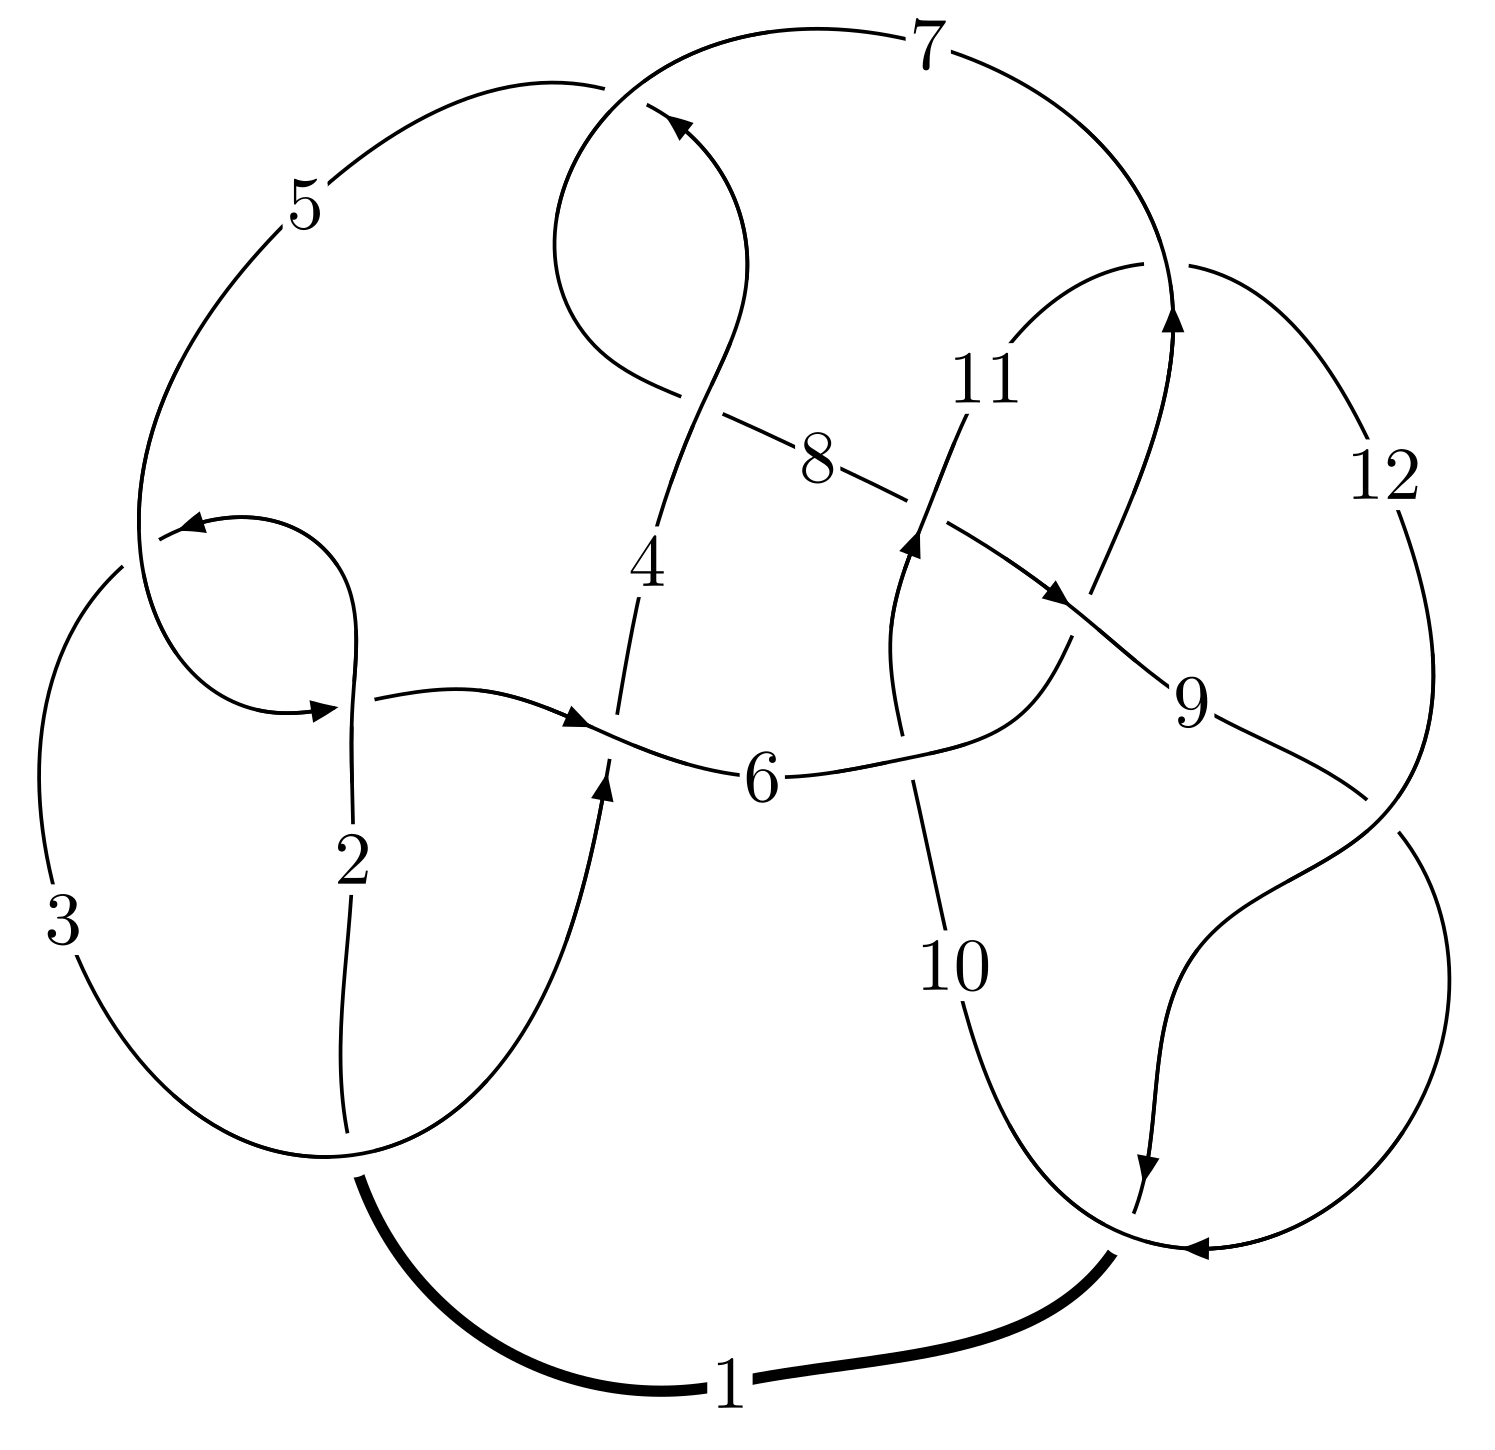
\includegraphics[width=112pt]{../../../GIT/diagram.site/Diagrams/png/2120_12n_0031.png}\\
\ \ \ A knot diagram\footnotemark}&
\allowdisplaybreaks
\textbf{Linearized knot diagam} \\
\cline{2-2}
 &
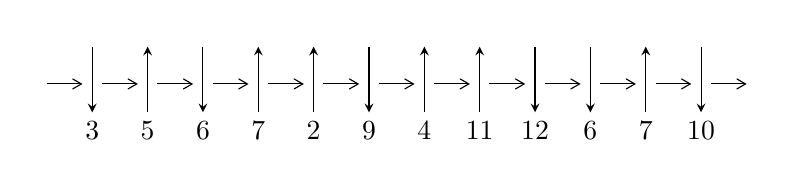
\begin{tikzpicture}[x=20pt, y=17pt]
	% nodes
	\node (C0) at (0, 0) {};
	\node (C1) at (1, 0) {};
	\node (C1U) at (1, +1) {};
	\node (C1D) at (1, -1) {3};

	\node (C2) at (2, 0) {};
	\node (C2U) at (2, +1) {};
	\node (C2D) at (2, -1) {5};

	\node (C3) at (3, 0) {};
	\node (C3U) at (3, +1) {};
	\node (C3D) at (3, -1) {6};

	\node (C4) at (4, 0) {};
	\node (C4U) at (4, +1) {};
	\node (C4D) at (4, -1) {7};

	\node (C5) at (5, 0) {};
	\node (C5U) at (5, +1) {};
	\node (C5D) at (5, -1) {2};

	\node (C6) at (6, 0) {};
	\node (C6U) at (6, +1) {};
	\node (C6D) at (6, -1) {9};

	\node (C7) at (7, 0) {};
	\node (C7U) at (7, +1) {};
	\node (C7D) at (7, -1) {4};

	\node (C8) at (8, 0) {};
	\node (C8U) at (8, +1) {};
	\node (C8D) at (8, -1) {11};

	\node (C9) at (9, 0) {};
	\node (C9U) at (9, +1) {};
	\node (C9D) at (9, -1) {12};

	\node (C10) at (10, 0) {};
	\node (C10U) at (10, +1) {};
	\node (C10D) at (10, -1) {6};

	\node (C11) at (11, 0) {};
	\node (C11U) at (11, +1) {};
	\node (C11D) at (11, -1) {7};

	\node (C12) at (12, 0) {};
	\node (C12U) at (12, +1) {};
	\node (C12D) at (12, -1) {10};
	\node (C13) at (13, 0) {};

	% arrows
	\draw[->,>={angle 60}]
	(C0) edge (C1) (C1) edge (C2) (C2) edge (C3) (C3) edge (C4) (C4) edge (C5) (C5) edge (C6) (C6) edge (C7) (C7) edge (C8) (C8) edge (C9) (C9) edge (C10) (C10) edge (C11) (C11) edge (C12) (C12) edge (C13) ;	\draw[->,>=stealth]
	(C1U) edge (C1D) (C2D) edge (C2U) (C3U) edge (C3D) (C4D) edge (C4U) (C5D) edge (C5U) (C6U) edge (C6D) (C7D) edge (C7U) (C8D) edge (C8U) (C9U) edge (C9D) (C10U) edge (C10D) (C11D) edge (C11U) (C12U) edge (C12D) ;
	\end{tikzpicture} \\
\hhline{~~} \\& 
\textbf{Solving Sequence} \\ \cline{2-2} 
 &
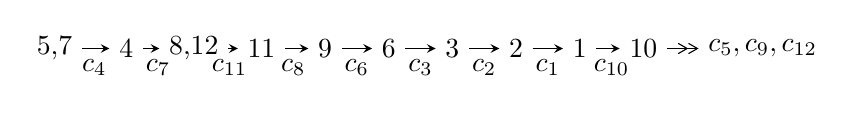
\begin{tikzpicture}[x=23pt, y=7pt]
	% node
	\node (A0) at (-1/8, 0) {5,7};
	\node (A1) at (1, 0) {4};
	\node (A2) at (33/16, 0) {8,12};
	\node (A3) at (25/8, 0) {11};
	\node (A4) at (33/8, 0) {9};
	\node (A5) at (41/8, 0) {6};
	\node (A6) at (49/8, 0) {3};
	\node (A7) at (57/8, 0) {2};
	\node (A8) at (65/8, 0) {1};
	\node (A9) at (73/8, 0) {10};
	\node (C1) at (1/2, -1) {$c_{4}$};
	\node (C2) at (3/2, -1) {$c_{7}$};
	\node (C3) at (21/8, -1) {$c_{11}$};
	\node (C4) at (29/8, -1) {$c_{8}$};
	\node (C5) at (37/8, -1) {$c_{6}$};
	\node (C6) at (45/8, -1) {$c_{3}$};
	\node (C7) at (53/8, -1) {$c_{2}$};
	\node (C8) at (61/8, -1) {$c_{1}$};
	\node (C9) at (69/8, -1) {$c_{10}$};
	\node (A10) at (11, 0) {$c_{5},c_{9},c_{12}$};

	% edge
	\draw[->,>=stealth]	
	(A0) edge (A1) (A1) edge (A2) (A2) edge (A3) (A3) edge (A4) (A4) edge (A5) (A5) edge (A6) (A6) edge (A7) (A7) edge (A8) (A8) edge (A9) ;
	\draw[->>,>={angle 60}]	
	(A9) edge (A10);
\end{tikzpicture} \\ 

\end{tabular} \\

\footnotetext{
The image of knot diagram is generated by the software ``\textbf{Draw programme}" developed by Andrew Bartholomew(\url{http://www.layer8.co.uk/maths/draw/index.htm\#Running-draw}), where we modified some parts for our purpose(\url{https://github.com/CATsTAILs/LinksPainter}).
}\phantom \\ \newline 
\centering \textbf{Ideals for irreducible components\footnotemark of $X_{\text{par}}$} 
 
\begin{align*}
I^u_{1}&=\langle 
1.28889\times10^{59} u^{23}-1.73916\times10^{59} u^{22}+\cdots+2.88300\times10^{61} b-2.28440\times10^{62},\\
\phantom{I^u_{1}}&\phantom{= \langle  }7.35803\times10^{59} u^{23}-1.22890\times10^{60} u^{22}+\cdots+5.76599\times10^{61} a-1.59769\times10^{63},\\
\phantom{I^u_{1}}&\phantom{= \langle  }u^{24}-2 u^{23}+\cdots-7168 u+1024\rangle \\
I^u_{2}&=\langle 
u^2+b- u+1,\;u^2+a- u+1,\;u^4+u^2+u+1\rangle \\
I^u_{3}&=\langle 
-2 u^5-3 u^3+u^2+b-2 u+2,\;-2 u^5-3 u^3+u^2+a-2 u+2,\;u^6- u^5+2 u^4-2 u^3+2 u^2-2 u+1\rangle \\
\\
I^v_{1}&=\langle 
a,\;1523 v^9+2050 v^8+\cdots+3335 b+8448,\\
\phantom{I^v_{1}}&\phantom{= \langle  }v^{10}+v^9-7 v^8+2 v^7+58 v^6+19 v^5-16 v^4-7 v^3+6 v^2+3 v+1\rangle \\
\end{align*}
\raggedright * 4 irreducible components of $\dim_{\mathbb{C}}=0$, with total 44 representations.\\
\footnotetext{All coefficients of polynomials are rational numbers. But the coefficients are sometimes approximated in decimal forms when there is not enough margin.}
\newpage
\renewcommand{\arraystretch}{1}
\centering \section*{I. $I^u_{1}= \langle 1.29\times10^{59} u^{23}-1.74\times10^{59} u^{22}+\cdots+2.88\times10^{61} b-2.28\times10^{62},\;7.36\times10^{59} u^{23}-1.23\times10^{60} u^{22}+\cdots+5.77\times10^{61} a-1.60\times10^{63},\;u^{24}-2 u^{23}+\cdots-7168 u+1024 \rangle$}
\flushleft \textbf{(i) Arc colorings}\\
\begin{tabular}{m{7pt} m{180pt} m{7pt} m{180pt} }
\flushright $a_{5}=$&$\begin{pmatrix}1\\0\end{pmatrix}$ \\
\flushright $a_{7}=$&$\begin{pmatrix}0\\u\end{pmatrix}$ \\
\flushright $a_{4}=$&$\begin{pmatrix}1\\u^2\end{pmatrix}$ \\
\flushright $a_{8}=$&$\begin{pmatrix}u\\u^3+u\end{pmatrix}$ \\
\flushright $a_{12}=$&$\begin{pmatrix}-0.0127611 u^{23}+0.0213129 u^{22}+\cdots-146.902 u+27.7088\\-0.00447065 u^{23}+0.00603249 u^{22}+\cdots-37.8270 u+7.92371\end{pmatrix}$ \\
\flushright $a_{11}=$&$\begin{pmatrix}-0.0127611 u^{23}+0.0213129 u^{22}+\cdots-146.902 u+27.7088\\-0.00460868 u^{23}+0.00759863 u^{22}+\cdots-54.9313 u+12.2340\end{pmatrix}$ \\
\flushright $a_{9}=$&$\begin{pmatrix}0.0184954 u^{23}-0.0271361 u^{22}+\cdots+171.538 u-29.5518\\0.00880936 u^{23}-0.00909508 u^{22}+\cdots+38.6739 u-3.95155\end{pmatrix}$ \\
\flushright $a_{6}=$&$\begin{pmatrix}0.00328632 u^{23}-0.00596273 u^{22}+\cdots+41.3269 u-7.17877\\-0.00508827 u^{23}+0.00785301 u^{22}+\cdots-54.7848 u+10.3149\end{pmatrix}$ \\
\flushright $a_{3}=$&$\begin{pmatrix}0.0000553993 u^{23}+0.0000911467 u^{22}+\cdots+0.275591 u+0.984609\\-0.000298497 u^{23}+0.00144194 u^{22}+\cdots-10.6087 u+2.48202\end{pmatrix}$ \\
\flushright $a_{2}=$&$\begin{pmatrix}0.000353896 u^{23}-0.00135079 u^{22}+\cdots+10.8843 u-1.49741\\-0.000298497 u^{23}+0.00144194 u^{22}+\cdots-10.6087 u+2.48202\end{pmatrix}$ \\
\flushright $a_{1}=$&$\begin{pmatrix}0.00774850 u^{23}-0.0135211 u^{22}+\cdots+97.1183 u-18.1182\\0.00446218 u^{23}-0.00755839 u^{22}+\cdots+55.7915 u-10.9394\end{pmatrix}$ \\
\flushright $a_{10}=$&$\begin{pmatrix}-0.00105139 u^{23}+0.00330070 u^{22}+\cdots-27.5679 u+6.56444\\0.00223494 u^{23}-0.00266203 u^{22}+\cdots+13.7590 u-0.614331\end{pmatrix}$\\&\end{tabular}
\flushleft \textbf{(ii) Obstruction class $= -1$}\\~\\
\flushleft \textbf{(iii) Cusp Shapes $= -0.0413329 u^{23}+0.0683918 u^{22}+\cdots-470.295 u+85.7076$}\\~\\
\newpage\renewcommand{\arraystretch}{1}
\flushleft \textbf{(iv) u-Polynomials at the component}\newline \\
\begin{tabular}{m{50pt}|m{274pt}}
Crossings & \hspace{64pt}u-Polynomials at each crossing \\
\hline $$\begin{aligned}c_{1}\end{aligned}$$&$\begin{aligned}
&u^{24}+3 u^{23}+\cdots-8 u+1
\end{aligned}$\\
\hline $$\begin{aligned}c_{2},c_{5}\end{aligned}$$&$\begin{aligned}
&u^{24}+7 u^{23}+\cdots+4 u+1
\end{aligned}$\\
\hline $$\begin{aligned}c_{3}\end{aligned}$$&$\begin{aligned}
&u^{24}-7 u^{23}+\cdots+155372 u+47236
\end{aligned}$\\
\hline $$\begin{aligned}c_{4},c_{7}\end{aligned}$$&$\begin{aligned}
&u^{24}+2 u^{23}+\cdots+7168 u+1024
\end{aligned}$\\
\hline $$\begin{aligned}c_{6}\end{aligned}$$&$\begin{aligned}
&u^{24}-4 u^{23}+\cdots-3 u+1
\end{aligned}$\\
\hline $$\begin{aligned}c_{8}\end{aligned}$$&$\begin{aligned}
&u^{24}+u^{23}+\cdots-5120 u+1024
\end{aligned}$\\
\hline $$\begin{aligned}c_{9},c_{12}\end{aligned}$$&$\begin{aligned}
&u^{24}-13 u^{23}+\cdots-2 u+1
\end{aligned}$\\
\hline $$\begin{aligned}c_{10}\end{aligned}$$&$\begin{aligned}
&u^{24}+4 u^{23}+\cdots-3009503 u+1672193
\end{aligned}$\\
\hline $$\begin{aligned}c_{11}\end{aligned}$$&$\begin{aligned}
&u^{24}-2 u^{23}+\cdots+2185 u+1831
\end{aligned}$\\
\hline
\end{tabular}\\~\\
\newpage\renewcommand{\arraystretch}{1}
\flushleft \textbf{(v) Riley Polynomials at the component}\newline \\
\begin{tabular}{m{50pt}|m{274pt}}
Crossings & \hspace{64pt}Riley Polynomials at each crossing \\
\hline $$\begin{aligned}c_{1}\end{aligned}$$&$\begin{aligned}
&y^{24}+43 y^{23}+\cdots+60 y+1
\end{aligned}$\\
\hline $$\begin{aligned}c_{2},c_{5}\end{aligned}$$&$\begin{aligned}
&y^{24}+3 y^{23}+\cdots-8 y+1
\end{aligned}$\\
\hline $$\begin{aligned}c_{3}\end{aligned}$$&$\begin{aligned}
&y^{24}+107 y^{23}+\cdots-359116296 y+2231239696
\end{aligned}$\\
\hline $$\begin{aligned}c_{4},c_{7}\end{aligned}$$&$\begin{aligned}
&y^{24}-30 y^{23}+\cdots-3145728 y+1048576
\end{aligned}$\\
\hline $$\begin{aligned}c_{6}\end{aligned}$$&$\begin{aligned}
&y^{24}+30 y^{22}+\cdots+y+1
\end{aligned}$\\
\hline $$\begin{aligned}c_{8}\end{aligned}$$&$\begin{aligned}
&y^{24}-57 y^{23}+\cdots-1572864 y+1048576
\end{aligned}$\\
\hline $$\begin{aligned}c_{9},c_{12}\end{aligned}$$&$\begin{aligned}
&y^{24}-27 y^{23}+\cdots-198 y+1
\end{aligned}$\\
\hline $$\begin{aligned}c_{10}\end{aligned}$$&$\begin{aligned}
&y^{24}+132 y^{23}+\cdots+20945455419869 y+2796229429249
\end{aligned}$\\
\hline $$\begin{aligned}c_{11}\end{aligned}$$&$\begin{aligned}
&y^{24}+20 y^{23}+\cdots+72680737 y+3352561
\end{aligned}$\\
\hline
\end{tabular}\\~\\
\newpage\flushleft \textbf{(vi) Complex Volumes and Cusp Shapes}
$$\begin{array}{c|c|c}  
\text{Solutions to }I^u_{1}& \I (\text{vol} + \sqrt{-1}CS) & \text{Cusp shape}\\
 \hline 
\begin{aligned}
u &= \phantom{-}1.028680 + 0.626726 I \\
a &= -0.533680 - 0.903018 I \\
b &= \phantom{-}0.034700 + 0.150384 I\end{aligned}
 & -5.30004 + 7.06597 I & -3.39619 - 6.37751 I \\ \hline\begin{aligned}
u &= \phantom{-}1.028680 - 0.626726 I \\
a &= -0.533680 + 0.903018 I \\
b &= \phantom{-}0.034700 - 0.150384 I\end{aligned}
 & -5.30004 - 7.06597 I & -3.39619 + 6.37751 I \\ \hline\begin{aligned}
u &= -0.497474 + 0.507669 I \\
a &= -0.361926 + 0.349425 I \\
b &= -0.008032 + 0.687395 I\end{aligned}
 & \phantom{-}0.84077 - 1.37467 I & \phantom{-}5.35239 + 4.26754 I \\ \hline\begin{aligned}
u &= -0.497474 - 0.507669 I \\
a &= -0.361926 - 0.349425 I \\
b &= -0.008032 - 0.687395 I\end{aligned}
 & \phantom{-}0.84077 + 1.37467 I & \phantom{-}5.35239 - 4.26754 I \\ \hline\begin{aligned}
u &= \phantom{-}0.551207 + 0.395512 I \\
a &= \phantom{-}0.685914 + 0.546768 I \\
b &= \phantom{-}0.865249 + 1.020670 I\end{aligned}
 & -0.14272 - 2.78886 I & \phantom{-}1.24898 + 0.91559 I \\ \hline\begin{aligned}
u &= \phantom{-}0.551207 - 0.395512 I \\
a &= \phantom{-}0.685914 - 0.546768 I \\
b &= \phantom{-}0.865249 - 1.020670 I\end{aligned}
 & -0.14272 + 2.78886 I & \phantom{-}1.24898 - 0.91559 I \\ \hline\begin{aligned}
u &= \phantom{-}0.534930 + 0.187354 I \\
a &= \phantom{-}1.80358 + 1.02511 I \\
b &= \phantom{-}2.21805 - 0.06958 I\end{aligned}
 & -2.26240 + 2.45863 I & -0.58956 - 2.80745 I \\ \hline\begin{aligned}
u &= \phantom{-}0.534930 - 0.187354 I \\
a &= \phantom{-}1.80358 - 1.02511 I \\
b &= \phantom{-}2.21805 + 0.06958 I\end{aligned}
 & -2.26240 - 2.45863 I & -0.58956 + 2.80745 I \\ \hline\begin{aligned}
u &= -0.53073 + 1.35148 I \\
a &= -0.444245 + 1.037430 I \\
b &= -0.185137 + 0.065890 I\end{aligned}
 & -5.91731 + 1.32680 I & -4.55064 - 0.68264 I \\ \hline\begin{aligned}
u &= -0.53073 - 1.35148 I \\
a &= -0.444245 - 1.037430 I \\
b &= -0.185137 - 0.065890 I\end{aligned}
 & -5.91731 - 1.32680 I & -4.55064 + 0.68264 I\\
 \hline 
 \end{array}$$\newpage$$\begin{array}{c|c|c}  
\text{Solutions to }I^u_{1}& \I (\text{vol} + \sqrt{-1}CS) & \text{Cusp shape}\\
 \hline 
\begin{aligned}
u &= -0.099117 + 0.535999 I \\
a &= -1.273020 - 0.388430 I \\
b &= \phantom{-}0.037166 + 0.328529 I\end{aligned}
 & \phantom{-}0.00212 - 1.46917 I & \phantom{-}0.28384 + 4.39333 I \\ \hline\begin{aligned}
u &= -0.099117 - 0.535999 I \\
a &= -1.273020 + 0.388430 I \\
b &= \phantom{-}0.037166 - 0.328529 I\end{aligned}
 & \phantom{-}0.00212 + 1.46917 I & \phantom{-}0.28384 - 4.39333 I \\ \hline\begin{aligned}
u &= \phantom{-}0.465375 + 0.278294 I \\
a &= -0.377175 + 0.887793 I \\
b &= \phantom{-}1.55399 + 0.43926 I\end{aligned}
 & -2.60162 - 0.06406 I & -5.33602 - 1.30009 I \\ \hline\begin{aligned}
u &= \phantom{-}0.465375 - 0.278294 I \\
a &= -0.377175 - 0.887793 I \\
b &= \phantom{-}1.55399 - 0.43926 I\end{aligned}
 & -2.60162 + 0.06406 I & -5.33602 + 1.30009 I \\ \hline\begin{aligned}
u &= -0.48281 + 2.18987 I \\
a &= \phantom{-}1.45037 - 0.79279 I \\
b &= \phantom{-}2.00018 - 0.40996 I\end{aligned}
 & \phantom{-}0.03963 - 1.93559 I & \phantom{-}3.24137 + 4.51519 I \\ \hline\begin{aligned}
u &= -0.48281 - 2.18987 I \\
a &= \phantom{-}1.45037 + 0.79279 I \\
b &= \phantom{-}2.00018 + 0.40996 I\end{aligned}
 & \phantom{-}0.03963 + 1.93559 I & \phantom{-}3.24137 - 4.51519 I \\ \hline\begin{aligned}
u &= -2.10598 + 1.47278 I \\
a &= \phantom{-}0.737984 - 0.025578 I \\
b &= \phantom{-}1.81967 - 0.11260 I\end{aligned}
 & \phantom{-}13.6003 - 6.5164 I & \phantom{-0.000000 } 0 \\ \hline\begin{aligned}
u &= -2.10598 - 1.47278 I \\
a &= \phantom{-}0.737984 + 0.025578 I \\
b &= \phantom{-}1.81967 + 0.11260 I\end{aligned}
 & \phantom{-}13.6003 + 6.5164 I & \phantom{-0.000000 } 0 \\ \hline\begin{aligned}
u &= \phantom{-}2.04936 + 1.71103 I \\
a &= \phantom{-}1.027290 + 0.232987 I \\
b &= \phantom{-}2.09607 + 0.15606 I\end{aligned}
 & \phantom{-}13.5215 + 14.1664 I & \phantom{-0.000000 } 0 \\ \hline\begin{aligned}
u &= \phantom{-}2.04936 - 1.71103 I \\
a &= \phantom{-}1.027290 - 0.232987 I \\
b &= \phantom{-}2.09607 - 0.15606 I\end{aligned}
 & \phantom{-}13.5215 - 14.1664 I & \phantom{-0.000000 } 0\\
 \hline 
 \end{array}$$\newpage$$\begin{array}{c|c|c}  
\text{Solutions to }I^u_{1}& \I (\text{vol} + \sqrt{-1}CS) & \text{Cusp shape}\\
 \hline 
\begin{aligned}
u &= \phantom{-}3.44120 + 1.32166 I \\
a &= -0.751676 + 0.034514 I \\
b &= -1.93632 - 0.01972 I\end{aligned}
 & \phantom{-}15.2941 - 1.5620 I & \phantom{-0.000000 } 0 \\ \hline\begin{aligned}
u &= \phantom{-}3.44120 - 1.32166 I \\
a &= -0.751676 - 0.034514 I \\
b &= -1.93632 + 0.01972 I\end{aligned}
 & \phantom{-}15.2941 + 1.5620 I & \phantom{-0.000000 } 0 \\ \hline\begin{aligned}
u &= -3.35464 + 2.16681 I \\
a &= -0.963420 + 0.242424 I \\
b &= -1.99558 + 0.06976 I\end{aligned}
 & \phantom{-}15.6939 - 6.0170 I & \phantom{-0.000000 } 0 \\ \hline\begin{aligned}
u &= -3.35464 - 2.16681 I \\
a &= -0.963420 - 0.242424 I \\
b &= -1.99558 - 0.06976 I\end{aligned}
 & \phantom{-}15.6939 + 6.0170 I & \phantom{-0.000000 } 0\\
 \hline 
 \end{array}$$\newpage\newpage\renewcommand{\arraystretch}{1}
\centering \section*{II. $I^u_{2}= \langle u^2+b- u+1,\;u^2+a- u+1,\;u^4+u^2+u+1 \rangle$}
\flushleft \textbf{(i) Arc colorings}\\
\begin{tabular}{m{7pt} m{180pt} m{7pt} m{180pt} }
\flushright $a_{5}=$&$\begin{pmatrix}1\\0\end{pmatrix}$ \\
\flushright $a_{7}=$&$\begin{pmatrix}0\\u\end{pmatrix}$ \\
\flushright $a_{4}=$&$\begin{pmatrix}1\\u^2\end{pmatrix}$ \\
\flushright $a_{8}=$&$\begin{pmatrix}u\\u^3+u\end{pmatrix}$ \\
\flushright $a_{12}=$&$\begin{pmatrix}- u^2+u-1\\- u^2+u-1\end{pmatrix}$ \\
\flushright $a_{11}=$&$\begin{pmatrix}- u^2+u-1\\u^3- u^2+2 u\end{pmatrix}$ \\
\flushright $a_{9}=$&$\begin{pmatrix}u\\u^3+u\end{pmatrix}$ \\
\flushright $a_{6}=$&$\begin{pmatrix}u^3\\- u^2\end{pmatrix}$ \\
\flushright $a_{3}=$&$\begin{pmatrix}u^3+u^2+1\\- u\end{pmatrix}$ \\
\flushright $a_{2}=$&$\begin{pmatrix}u^3+u^2+u+1\\- u\end{pmatrix}$ \\
\flushright $a_{1}=$&$\begin{pmatrix}- u\\- u^3- u\end{pmatrix}$ \\
\flushright $a_{10}=$&$\begin{pmatrix}- u^2+2 u-1\\u^3- u^2+2 u-1\end{pmatrix}$\\&\end{tabular}
\flushleft \textbf{(ii) Obstruction class $= 1$}\\~\\
\flushleft \textbf{(iii) Cusp Shapes $= - u^3-6 u^2-2 u-7$}\\~\\
\newpage\renewcommand{\arraystretch}{1}
\flushleft \textbf{(iv) u-Polynomials at the component}\newline \\
\begin{tabular}{m{50pt}|m{274pt}}
Crossings & \hspace{64pt}u-Polynomials at each crossing \\
\hline $$\begin{aligned}c_{1},c_{6}\end{aligned}$$&$\begin{aligned}
&u^4-2 u^3+3 u^2- u+1
\end{aligned}$\\
\hline $$\begin{aligned}c_{2},c_{4}\end{aligned}$$&$\begin{aligned}
&u^4+u^2+u+1
\end{aligned}$\\
\hline $$\begin{aligned}c_{3}\end{aligned}$$&$\begin{aligned}
&u^4+3 u^3+4 u^2+3 u+2
\end{aligned}$\\
\hline $$\begin{aligned}c_{5},c_{7}\end{aligned}$$&$\begin{aligned}
&u^4+u^2- u+1
\end{aligned}$\\
\hline $$\begin{aligned}c_{8}\end{aligned}$$&$\begin{aligned}
&u^4
\end{aligned}$\\
\hline $$\begin{aligned}c_{9}\end{aligned}$$&$\begin{aligned}
&(u-1)^4
\end{aligned}$\\
\hline $$\begin{aligned}c_{10},c_{11}\end{aligned}$$&$\begin{aligned}
&u^4- u^3+3 u^2-2 u+1
\end{aligned}$\\
\hline $$\begin{aligned}c_{12}\end{aligned}$$&$\begin{aligned}
&(u+1)^4
\end{aligned}$\\
\hline
\end{tabular}\\~\\
\newpage\renewcommand{\arraystretch}{1}
\flushleft \textbf{(v) Riley Polynomials at the component}\newline \\
\begin{tabular}{m{50pt}|m{274pt}}
Crossings & \hspace{64pt}Riley Polynomials at each crossing \\
\hline $$\begin{aligned}c_{1},c_{6}\end{aligned}$$&$\begin{aligned}
&y^4+2 y^3+7 y^2+5 y+1
\end{aligned}$\\
\hline $$\begin{aligned}c_{2},c_{4},c_{5}\\c_{7}\end{aligned}$$&$\begin{aligned}
&y^4+2 y^3+3 y^2+y+1
\end{aligned}$\\
\hline $$\begin{aligned}c_{3}\end{aligned}$$&$\begin{aligned}
&y^4- y^3+2 y^2+7 y+4
\end{aligned}$\\
\hline $$\begin{aligned}c_{8}\end{aligned}$$&$\begin{aligned}
&y^4
\end{aligned}$\\
\hline $$\begin{aligned}c_{9},c_{12}\end{aligned}$$&$\begin{aligned}
&(y-1)^4
\end{aligned}$\\
\hline $$\begin{aligned}c_{10},c_{11}\end{aligned}$$&$\begin{aligned}
&y^4+5 y^3+7 y^2+2 y+1
\end{aligned}$\\
\hline
\end{tabular}\\~\\
\newpage\flushleft \textbf{(vi) Complex Volumes and Cusp Shapes}
$$\begin{array}{c|c|c}  
\text{Solutions to }I^u_{2}& \I (\text{vol} + \sqrt{-1}CS) & \text{Cusp shape}\\
 \hline 
\begin{aligned}
u &= -0.547424 + 0.585652 I \\
a &= -1.50411 + 1.22685 I \\
b &= -1.50411 + 1.22685 I\end{aligned}
 & -0.66484 - 1.39709 I & -6.04449 + 2.35025 I \\ \hline\begin{aligned}
u &= -0.547424 - 0.585652 I \\
a &= -1.50411 - 1.22685 I \\
b &= -1.50411 - 1.22685 I\end{aligned}
 & -0.66484 + 1.39709 I & -6.04449 - 2.35025 I \\ \hline\begin{aligned}
u &= \phantom{-}0.547424 + 1.120870 I \\
a &= \phantom{-}0.504108 - 0.106312 I \\
b &= \phantom{-}0.504108 - 0.106312 I\end{aligned}
 & -4.26996 + 7.64338 I & -0.45551 - 9.20433 I \\ \hline\begin{aligned}
u &= \phantom{-}0.547424 - 1.120870 I \\
a &= \phantom{-}0.504108 + 0.106312 I \\
b &= \phantom{-}0.504108 + 0.106312 I\end{aligned}
 & -4.26996 - 7.64338 I & -0.45551 + 9.20433 I\\
 \hline 
 \end{array}$$\newpage\newpage\renewcommand{\arraystretch}{1}
\centering \section*{III. $I^u_{3}= \langle -2 u^5-3 u^3+u^2+b-2 u+2,\;-2 u^5-3 u^3+u^2+a-2 u+2,\;u^6- u^5+2 u^4-2 u^3+2 u^2-2 u+1 \rangle$}
\flushleft \textbf{(i) Arc colorings}\\
\begin{tabular}{m{7pt} m{180pt} m{7pt} m{180pt} }
\flushright $a_{5}=$&$\begin{pmatrix}1\\0\end{pmatrix}$ \\
\flushright $a_{7}=$&$\begin{pmatrix}0\\u\end{pmatrix}$ \\
\flushright $a_{4}=$&$\begin{pmatrix}1\\u^2\end{pmatrix}$ \\
\flushright $a_{8}=$&$\begin{pmatrix}u\\u^3+u\end{pmatrix}$ \\
\flushright $a_{12}=$&$\begin{pmatrix}2 u^5+3 u^3- u^2+2 u-2\\2 u^5+3 u^3- u^2+2 u-2\end{pmatrix}$ \\
\flushright $a_{11}=$&$\begin{pmatrix}2 u^5+3 u^3- u^2+2 u-2\\3 u^5- u^4+5 u^3-3 u^2+4 u-4\end{pmatrix}$ \\
\flushright $a_{9}=$&$\begin{pmatrix}u\\u^3+u\end{pmatrix}$ \\
\flushright $a_{6}=$&$\begin{pmatrix}u^3\\u^5+u^3+u\end{pmatrix}$ \\
\flushright $a_{3}=$&$\begin{pmatrix}- u^5+u^4-2 u^3+2 u^2-2 u+2\\- u^5-2 u^3+u^2- u+1\end{pmatrix}$ \\
\flushright $a_{2}=$&$\begin{pmatrix}u^4+u^2- u+1\\- u^5-2 u^3+u^2- u+1\end{pmatrix}$ \\
\flushright $a_{1}=$&$\begin{pmatrix}- u\\- u^3- u\end{pmatrix}$ \\
\flushright $a_{10}=$&$\begin{pmatrix}2 u^5+3 u^3- u^2+3 u-2\\2 u^5+4 u^3- u^2+3 u-2\end{pmatrix}$\\&\end{tabular}
\flushleft \textbf{(ii) Obstruction class $= 1$}\\~\\
\flushleft \textbf{(iii) Cusp Shapes $= -3 u^5+u^4+4 u^2+3 u+1$}\\~\\
\newpage\renewcommand{\arraystretch}{1}
\flushleft \textbf{(iv) u-Polynomials at the component}\newline \\
\begin{tabular}{m{50pt}|m{274pt}}
Crossings & \hspace{64pt}u-Polynomials at each crossing \\
\hline $$\begin{aligned}c_{1},c_{6}\end{aligned}$$&$\begin{aligned}
&u^6-3 u^5+4 u^4-2 u^3+1
\end{aligned}$\\
\hline $$\begin{aligned}c_{2},c_{4}\end{aligned}$$&$\begin{aligned}
&u^6- u^5+2 u^4-2 u^3+2 u^2-2 u+1
\end{aligned}$\\
\hline $$\begin{aligned}c_{3}\end{aligned}$$&$\begin{aligned}
&(u^3- u^2+1)^2
\end{aligned}$\\
\hline $$\begin{aligned}c_{5},c_{7}\end{aligned}$$&$\begin{aligned}
&u^6+u^5+2 u^4+2 u^3+2 u^2+2 u+1
\end{aligned}$\\
\hline $$\begin{aligned}c_{8}\end{aligned}$$&$\begin{aligned}
&u^6
\end{aligned}$\\
\hline $$\begin{aligned}c_{9}\end{aligned}$$&$\begin{aligned}
&(u-1)^6
\end{aligned}$\\
\hline $$\begin{aligned}c_{10},c_{11}\end{aligned}$$&$\begin{aligned}
&u^6-2 u^3+4 u^2-3 u+1
\end{aligned}$\\
\hline $$\begin{aligned}c_{12}\end{aligned}$$&$\begin{aligned}
&(u+1)^6
\end{aligned}$\\
\hline
\end{tabular}\\~\\
\newpage\renewcommand{\arraystretch}{1}
\flushleft \textbf{(v) Riley Polynomials at the component}\newline \\
\begin{tabular}{m{50pt}|m{274pt}}
Crossings & \hspace{64pt}Riley Polynomials at each crossing \\
\hline $$\begin{aligned}c_{1},c_{6}\end{aligned}$$&$\begin{aligned}
&y^6- y^5+4 y^4-2 y^3+8 y^2+1
\end{aligned}$\\
\hline $$\begin{aligned}c_{2},c_{4},c_{5}\\c_{7}\end{aligned}$$&$\begin{aligned}
&y^6+3 y^5+4 y^4+2 y^3+1
\end{aligned}$\\
\hline $$\begin{aligned}c_{3}\end{aligned}$$&$\begin{aligned}
&(y^3- y^2+2 y-1)^2
\end{aligned}$\\
\hline $$\begin{aligned}c_{8}\end{aligned}$$&$\begin{aligned}
&y^6
\end{aligned}$\\
\hline $$\begin{aligned}c_{9},c_{12}\end{aligned}$$&$\begin{aligned}
&(y-1)^6
\end{aligned}$\\
\hline $$\begin{aligned}c_{10},c_{11}\end{aligned}$$&$\begin{aligned}
&y^6+8 y^4-2 y^3+4 y^2- y+1
\end{aligned}$\\
\hline
\end{tabular}\\~\\
\newpage\flushleft \textbf{(vi) Complex Volumes and Cusp Shapes}
$$\begin{array}{c|c|c}  
\text{Solutions to }I^u_{3}& \I (\text{vol} + \sqrt{-1}CS) & \text{Cusp shape}\\
 \hline 
\begin{aligned}
u &= -0.498832 + 1.001300 I \\
a &= -0.702221 - 0.130845 I \\
b &= -0.702221 - 0.130845 I\end{aligned}
 & -1.91067 - 2.82812 I & -0.06063 + 4.05868 I \\ \hline\begin{aligned}
u &= -0.498832 - 1.001300 I \\
a &= -0.702221 + 0.130845 I \\
b &= -0.702221 + 0.130845 I\end{aligned}
 & -1.91067 + 2.82812 I & -0.06063 - 4.05868 I \\ \hline\begin{aligned}
u &= \phantom{-}0.284920 + 1.115140 I \\
a &= \phantom{-}0.447279 - 0.479689 I \\
b &= \phantom{-}0.447279 - 0.479689 I\end{aligned}
 & -6.04826\phantom{ +0.000000I} & -7.59911 + 2.50363 I \\ \hline\begin{aligned}
u &= \phantom{-}0.284920 - 1.115140 I \\
a &= \phantom{-}0.447279 + 0.479689 I \\
b &= \phantom{-}0.447279 + 0.479689 I\end{aligned}
 & -6.04826\phantom{ +0.000000I} & -7.59911 - 2.50363 I \\ \hline\begin{aligned}
u &= \phantom{-}0.713912 + 0.305839 I \\
a &= -0.74506 + 2.00027 I \\
b &= -0.74506 + 2.00027 I\end{aligned}
 & -1.91067 - 2.82812 I & \phantom{-}5.15973 + 2.26538 I \\ \hline\begin{aligned}
u &= \phantom{-}0.713912 - 0.305839 I \\
a &= -0.74506 - 2.00027 I \\
b &= -0.74506 - 2.00027 I\end{aligned}
 & -1.91067 + 2.82812 I & \phantom{-}5.15973 - 2.26538 I\\
 \hline 
 \end{array}$$\newpage\newpage\renewcommand{\arraystretch}{1}
\centering \section*{IV. $I^v_{1}= \langle a,\;1523 v^9+2050 v^8+\cdots+3335 b+8448,\;v^{10}+v^9+\cdots+3 v+1 \rangle$}
\flushleft \textbf{(i) Arc colorings}\\
\begin{tabular}{m{7pt} m{180pt} m{7pt} m{180pt} }
\flushright $a_{5}=$&$\begin{pmatrix}1\\0\end{pmatrix}$ \\
\flushright $a_{7}=$&$\begin{pmatrix}v\\0\end{pmatrix}$ \\
\flushright $a_{4}=$&$\begin{pmatrix}1\\0\end{pmatrix}$ \\
\flushright $a_{8}=$&$\begin{pmatrix}v\\0\end{pmatrix}$ \\
\flushright $a_{12}=$&$\begin{pmatrix}0\\-0.456672 v^{9}-0.614693 v^{8}+\cdots-5.06627 v-2.53313\end{pmatrix}$ \\
\flushright $a_{11}=$&$\begin{pmatrix}-0.158021 v^{9}-0.0569715 v^{8}+\cdots-0.930735 v-0.158021\\-0.456672 v^{9}-0.614693 v^{8}+\cdots-5.06627 v-2.53313\end{pmatrix}$ \\
\flushright $a_{9}=$&$\begin{pmatrix}0.117241 v^{9}+0.133433 v^{8}+\cdots+1.47736 v+0.117241\\0.125637 v^{9}+0.242879 v^{8}+\cdots+2.66207 v+1.33103\end{pmatrix}$ \\
\flushright $a_{6}=$&$\begin{pmatrix}0.178111 v^{9}+0.133433 v^{8}+\cdots+1.94693 v+0.178111\\0.286957 v^{9}+0.347826 v^{8}+\cdots+2.57391 v+1.28696\end{pmatrix}$ \\
\flushright $a_{3}=$&$\begin{pmatrix}-0.0932534 v^{9}+0.700750 v^{7}+\cdots-0.700750 v+1.44498\\-0.286957 v^{9}-0.347826 v^{8}+\cdots-2.57391 v-0.286957\end{pmatrix}$ \\
\flushright $a_{2}=$&$\begin{pmatrix}0.193703 v^{9}+0.347826 v^{8}+\cdots+1.87316 v+1.73193\\-0.286957 v^{9}-0.347826 v^{8}+\cdots-2.57391 v-0.286957\end{pmatrix}$ \\
\flushright $a_{1}=$&$\begin{pmatrix}-0.178111 v^{9}-0.133433 v^{8}+\cdots-1.94693 v-0.178111\\-0.286957 v^{9}-0.347826 v^{8}+\cdots-2.57391 v-1.28696\end{pmatrix}$ \\
\flushright $a_{10}=$&$\begin{pmatrix}0.117241 v^{9}+0.133433 v^{8}+\cdots+1.47736 v+0.117241\\-0.286957 v^{9}-0.347826 v^{8}+\cdots-2.57391 v-1.28696\end{pmatrix}$\\&\end{tabular}
\flushleft \textbf{(ii) Obstruction class $= 1$}\\~\\
\flushleft \textbf{(iii) Cusp Shapes $= -\frac{6289}{3335} v^9-\frac{14}{23} v^8+\frac{46278}{3335} v^7-\frac{43091}{3335} v^6-\frac{341636}{3335} v^5+\frac{22875}{667} v^4+\frac{72729}{3335} v^3+\frac{5464}{3335} v^2-\frac{48743}{3335} v-\frac{1839}{3335}$}\\~\\
\newpage\renewcommand{\arraystretch}{1}
\flushleft \textbf{(iv) u-Polynomials at the component}\newline \\
\begin{tabular}{m{50pt}|m{274pt}}
Crossings & \hspace{64pt}u-Polynomials at each crossing \\
\hline $$\begin{aligned}c_{1},c_{3},c_{5}\end{aligned}$$&$\begin{aligned}
&(u^2- u+1)^5
\end{aligned}$\\
\hline $$\begin{aligned}c_{2}\end{aligned}$$&$\begin{aligned}
&(u^2+u+1)^5
\end{aligned}$\\
\hline $$\begin{aligned}c_{4},c_{7}\end{aligned}$$&$\begin{aligned}
&u^{10}
\end{aligned}$\\
\hline $$\begin{aligned}c_{6}\end{aligned}$$&$\begin{aligned}
&(u^5-3 u^4+4 u^3- u^2- u+1)^2
\end{aligned}$\\
\hline $$\begin{aligned}c_{8}\end{aligned}$$&$\begin{aligned}
&(u^5- u^4+2 u^3- u^2+u-1)^2
\end{aligned}$\\
\hline $$\begin{aligned}c_{9}\end{aligned}$$&$\begin{aligned}
&(u^5+u^4-2 u^3- u^2+u-1)^2
\end{aligned}$\\
\hline $$\begin{aligned}c_{10},c_{12}\end{aligned}$$&$\begin{aligned}
&(u^5- u^4-2 u^3+u^2+u+1)^2
\end{aligned}$\\
\hline $$\begin{aligned}c_{11}\end{aligned}$$&$\begin{aligned}
&(u^5+u^4+2 u^3+u^2+u+1)^2
\end{aligned}$\\
\hline
\end{tabular}\\~\\
\newpage\renewcommand{\arraystretch}{1}
\flushleft \textbf{(v) Riley Polynomials at the component}\newline \\
\begin{tabular}{m{50pt}|m{274pt}}
Crossings & \hspace{64pt}Riley Polynomials at each crossing \\
\hline $$\begin{aligned}c_{1},c_{2},c_{3}\\c_{5}\end{aligned}$$&$\begin{aligned}
&(y^2+y+1)^5
\end{aligned}$\\
\hline $$\begin{aligned}c_{4},c_{7}\end{aligned}$$&$\begin{aligned}
&y^{10}
\end{aligned}$\\
\hline $$\begin{aligned}c_{6}\end{aligned}$$&$\begin{aligned}
&(y^5- y^4+8 y^3-3 y^2+3 y-1)^2
\end{aligned}$\\
\hline $$\begin{aligned}c_{8},c_{11}\end{aligned}$$&$\begin{aligned}
&(y^5+3 y^4+4 y^3+y^2- y-1)^2
\end{aligned}$\\
\hline $$\begin{aligned}c_{9},c_{10},c_{12}\end{aligned}$$&$\begin{aligned}
&(y^5-5 y^4+8 y^3-3 y^2- y-1)^2
\end{aligned}$\\
\hline
\end{tabular}\\~\\
\newpage\flushleft \textbf{(vi) Complex Volumes and Cusp Shapes}
$$\begin{array}{c|c|c}  
\text{Solutions to }I^v_{1}& \I (\text{vol} + \sqrt{-1}CS) & \text{Cusp shape}\\
 \hline 
\begin{aligned}
v &= \phantom{-}0.540263 + 0.316514 I \\
a &= \phantom{-0.000000 } 0 \\
b &= -1.13119 - 0.85946 I\end{aligned}
 & -0.329100 - 0.499304 I & -1.95395 + 0.91636 I \\ \hline\begin{aligned}
v &= \phantom{-}0.540263 - 0.316514 I \\
a &= \phantom{-0.000000 } 0 \\
b &= -1.13119 + 0.85946 I\end{aligned}
 & -0.329100 + 0.499304 I & -1.95395 - 0.91636 I \\ \hline\begin{aligned}
v &= -0.544240 + 0.309625 I \\
a &= \phantom{-0.000000 } 0 \\
b &= -0.17872 + 1.40938 I\end{aligned}
 & -0.32910 + 3.56046 I & -2.01870 - 9.75023 I \\ \hline\begin{aligned}
v &= -0.544240 - 0.309625 I \\
a &= \phantom{-0.000000 } 0 \\
b &= -0.17872 - 1.40938 I\end{aligned}
 & -0.32910 - 3.56046 I & -2.01870 + 9.75023 I \\ \hline\begin{aligned}
v &= -0.172885 + 0.299445 I \\
a &= \phantom{-0.000000 } 0 \\
b &= -1.10887 - 1.92062 I\end{aligned}
 & -2.40108 - 2.02988 I & \phantom{-}2.76075 - 3.67600 I \\ \hline\begin{aligned}
v &= -0.172885 - 0.299445 I \\
a &= \phantom{-0.000000 } 0 \\
b &= -1.10887 + 1.92062 I\end{aligned}
 & -2.40108 + 2.02988 I & \phantom{-}2.76075 + 3.67600 I \\ \hline\begin{aligned}
v &= \phantom{-}2.17384 + 1.62819 I \\
a &= \phantom{-0.000000 } 0 \\
b &= \phantom{-}0.399195 + 0.253095 I\end{aligned}
 & -5.87256 + 2.37095 I & -6.85700 - 6.98324 I \\ \hline\begin{aligned}
v &= \phantom{-}2.17384 - 1.62819 I \\
a &= \phantom{-0.000000 } 0 \\
b &= \phantom{-}0.399195 - 0.253095 I\end{aligned}
 & -5.87256 - 2.37095 I & -6.85700 + 6.98324 I \\ \hline\begin{aligned}
v &= -2.49698 + 1.06850 I \\
a &= \phantom{-0.000000 } 0 \\
b &= \phantom{-}0.019589 - 0.472260 I\end{aligned}
 & -5.87256 + 6.43072 I & -9.93110 - 1.72471 I \\ \hline\begin{aligned}
v &= -2.49698 - 1.06850 I \\
a &= \phantom{-0.000000 } 0 \\
b &= \phantom{-}0.019589 + 0.472260 I\end{aligned}
 & -5.87256 - 6.43072 I & -9.93110 + 1.72471 I\\
 \hline 
 \end{array}$$\newpage
\newpage\renewcommand{\arraystretch}{1}
\centering \section*{ V. u-Polynomials}
\begin{tabular}{m{50pt}|m{274pt}}
Crossings & \hspace{64pt}u-Polynomials at each crossing \\
\hline $$\begin{aligned}c_{1}\end{aligned}$$&$\begin{aligned}
&(u^2- u+1)^5(u^4-2 u^3+3 u^2- u+1)(u^6-3 u^5+4 u^4-2 u^3+1)\\
&\cdot(u^{24}+3 u^{23}+\cdots-8 u+1)
\end{aligned}$\\
\hline $$\begin{aligned}c_{2}\end{aligned}$$&$\begin{aligned}
&(u^2+u+1)^5(u^4+u^2+u+1)(u^6- u^5+2 u^4-2 u^3+2 u^2-2 u+1)\\
&\cdot(u^{24}+7 u^{23}+\cdots+4 u+1)
\end{aligned}$\\
\hline $$\begin{aligned}c_{3}\end{aligned}$$&$\begin{aligned}
&(u^2- u+1)^5(u^3- u^2+1)^2(u^4+3 u^3+4 u^2+3 u+2)\\
&\cdot(u^{24}-7 u^{23}+\cdots+155372 u+47236)
\end{aligned}$\\
\hline $$\begin{aligned}c_{4}\end{aligned}$$&$\begin{aligned}
&u^{10}(u^4+u^2+u+1)(u^6- u^5+2 u^4-2 u^3+2 u^2-2 u+1)\\
&\cdot(u^{24}+2 u^{23}+\cdots+7168 u+1024)
\end{aligned}$\\
\hline $$\begin{aligned}c_{5}\end{aligned}$$&$\begin{aligned}
&(u^2- u+1)^5(u^4+u^2- u+1)(u^6+u^5+2 u^4+2 u^3+2 u^2+2 u+1)\\
&\cdot(u^{24}+7 u^{23}+\cdots+4 u+1)
\end{aligned}$\\
\hline $$\begin{aligned}c_{6}\end{aligned}$$&$\begin{aligned}
&(u^4-2 u^3+3 u^2- u+1)(u^5-3 u^4+4 u^3- u^2- u+1)^2\\
&\cdot(u^6-3 u^5+4 u^4-2 u^3+1)(u^{24}-4 u^{23}+\cdots-3 u+1)
\end{aligned}$\\
\hline $$\begin{aligned}c_{7}\end{aligned}$$&$\begin{aligned}
&u^{10}(u^4+u^2- u+1)(u^6+u^5+2 u^4+2 u^3+2 u^2+2 u+1)\\
&\cdot(u^{24}+2 u^{23}+\cdots+7168 u+1024)
\end{aligned}$\\
\hline $$\begin{aligned}c_{8}\end{aligned}$$&$\begin{aligned}
&u^{10}(u^5- u^4+\cdots+u-1)^{2}(u^{24}+u^{23}+\cdots-5120 u+1024)
\end{aligned}$\\
\hline $$\begin{aligned}c_{9}\end{aligned}$$&$\begin{aligned}
&((u-1)^{10})(u^5+u^4+\cdots+u-1)^{2}(u^{24}-13 u^{23}+\cdots-2 u+1)
\end{aligned}$\\
\hline $$\begin{aligned}c_{10}\end{aligned}$$&$\begin{aligned}
&(u^4- u^3+3 u^2-2 u+1)(u^5- u^4-2 u^3+u^2+u+1)^2\\
&\cdot(u^6-2 u^3+4 u^2-3 u+1)(u^{24}+4 u^{23}+\cdots-3009503 u+1672193)
\end{aligned}$\\
\hline $$\begin{aligned}c_{11}\end{aligned}$$&$\begin{aligned}
&(u^4- u^3+3 u^2-2 u+1)(u^5+u^4+2 u^3+u^2+u+1)^2\\
&\cdot(u^6-2 u^3+4 u^2-3 u+1)(u^{24}-2 u^{23}+\cdots+2185 u+1831)
\end{aligned}$\\
\hline $$\begin{aligned}c_{12}\end{aligned}$$&$\begin{aligned}
&((u+1)^{10})(u^5- u^4+\cdots+u+1)^{2}(u^{24}-13 u^{23}+\cdots-2 u+1)
\end{aligned}$\\
\hline
\end{tabular}\newpage\renewcommand{\arraystretch}{1}
\centering \section*{ VI. Riley Polynomials}
\begin{tabular}{m{50pt}|m{274pt}}
Crossings & \hspace{64pt}Riley Polynomials at each crossing \\
\hline $$\begin{aligned}c_{1}\end{aligned}$$&$\begin{aligned}
&((y^2+y+1)^5)(y^4+2 y^3+\cdots+5 y+1)(y^6- y^5+\cdots+8 y^2+1)\\
&\cdot(y^{24}+43 y^{23}+\cdots+60 y+1)
\end{aligned}$\\
\hline $$\begin{aligned}c_{2},c_{5}\end{aligned}$$&$\begin{aligned}
&(y^2+y+1)^5(y^4+2 y^3+3 y^2+y+1)(y^6+3 y^5+4 y^4+2 y^3+1)\\
&\cdot(y^{24}+3 y^{23}+\cdots-8 y+1)
\end{aligned}$\\
\hline $$\begin{aligned}c_{3}\end{aligned}$$&$\begin{aligned}
&(y^2+y+1)^5(y^3- y^2+2 y-1)^2(y^4- y^3+2 y^2+7 y+4)\\
&\cdot(y^{24}+107 y^{23}+\cdots-359116296 y+2231239696)
\end{aligned}$\\
\hline $$\begin{aligned}c_{4},c_{7}\end{aligned}$$&$\begin{aligned}
&y^{10}(y^4+2 y^3+3 y^2+y+1)(y^6+3 y^5+4 y^4+2 y^3+1)\\
&\cdot(y^{24}-30 y^{23}+\cdots-3145728 y+1048576)
\end{aligned}$\\
\hline $$\begin{aligned}c_{6}\end{aligned}$$&$\begin{aligned}
&(y^4+2 y^3+7 y^2+5 y+1)(y^5- y^4+8 y^3-3 y^2+3 y-1)^2\\
&\cdot(y^6- y^5+4 y^4-2 y^3+8 y^2+1)(y^{24}+30 y^{22}+\cdots+y+1)
\end{aligned}$\\
\hline $$\begin{aligned}c_{8}\end{aligned}$$&$\begin{aligned}
&y^{10}(y^5+3 y^4+4 y^3+y^2- y-1)^2\\
&\cdot(y^{24}-57 y^{23}+\cdots-1572864 y+1048576)
\end{aligned}$\\
\hline $$\begin{aligned}c_{9},c_{12}\end{aligned}$$&$\begin{aligned}
&(y-1)^{10}(y^5-5 y^4+8 y^3-3 y^2- y-1)^2\\
&\cdot(y^{24}-27 y^{23}+\cdots-198 y+1)
\end{aligned}$\\
\hline $$\begin{aligned}c_{10}\end{aligned}$$&$\begin{aligned}
&(y^4+5 y^3+7 y^2+2 y+1)(y^5-5 y^4+8 y^3-3 y^2- y-1)^2\\
&\cdot(y^6+8 y^4-2 y^3+4 y^2- y+1)\\
&\cdot(y^{24}+132 y^{23}+\cdots+20945455419869 y+2796229429249)
\end{aligned}$\\
\hline $$\begin{aligned}c_{11}\end{aligned}$$&$\begin{aligned}
&(y^4+5 y^3+7 y^2+2 y+1)(y^5+3 y^4+4 y^3+y^2- y-1)^2\\
&\cdot(y^6+8 y^4-2 y^3+4 y^2- y+1)\\
&\cdot(y^{24}+20 y^{23}+\cdots+72680737 y+3352561)
\end{aligned}$\\
\hline
\end{tabular}
\vskip 2pc
\end{document}